\chapter{Materials And Methods}
\section{HC18 Dataset}
\subsection{Description}
\noindent

	The collection of 1334 2D ultrasound images of fetal head were collected from the database of the Department of Obstetrics of the Radboud University Medical Center, Nijmegen, the Netherlands. All of the fetal head ultrasound images for this challenge were captured in the standard plane which is the specifically used to measure the HC \cite{thomas}.

	The data is divided into a training set of 999 images and a test set of 335 images. The size of each 2D ultrasound image is 800x540 pixel with a pixel size ranging from 0.052 to 0.326 mm. The information of pixel of each image can be found in the CSV files: ‘training-set-pixel-size-and-HC.csv’ and ‘test-set-pixel-size.csv’. The variability of pixel size was resulted from the adjustment of sonographers during examinations which led to a different shape and size of the fetal heads. In addition, in the training set, come along with each ultrasound image is a manual annotation in millimeters. All of the image file-names start with a number. However, the file-names only set to 805 because some images were come from the same examination (different frame during monitoring), therefore they have a similar appearance \cite{thomas}.
	
	\begin{figure}[H]
		\centering
		\subcaptionbox{A fetal head ultrasound image.}{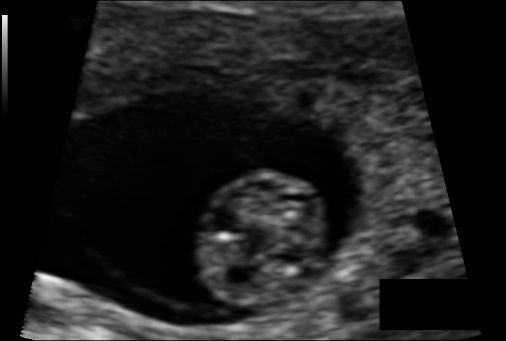
\includegraphics[width=0.45\textwidth]{./hinhanh/chap3/us_image.png}}%
		\hfill % <-- Seperation
		\subcaptionbox{An annotation  created by sonographers.}{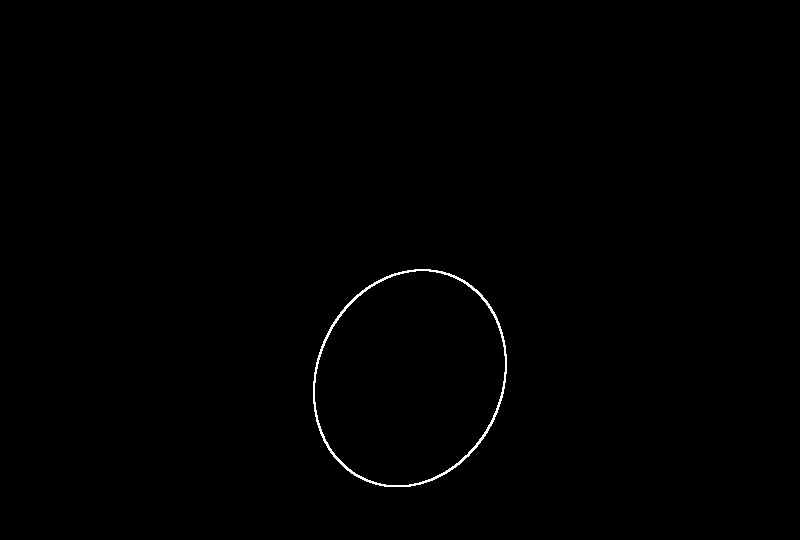
\includegraphics[width=0.45\textwidth]{./hinhanh/chap3/ori_annotation.png}}%
		\hfill % <-- Seperation
		\caption{HC-18 dataset sample.}
	\end{figure}

	

\subsection{Pre-processing}
\noindent

	During each examination, the sonographer manually draws an ellipse which best fit the fetal head and save it as annotation of the ultrasound image. And based on these annotations, we apply a few image processing to extract the ellipse coordinates and created a dataset in COCO format for further training methods.
	
	\begin{figure}[H]
		\centering
		\subcaptionbox{a processed annotation}{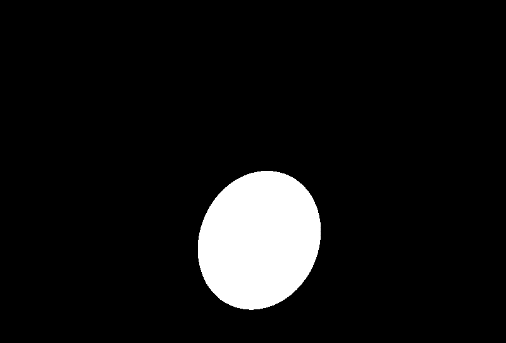
\includegraphics[width=0.45\textwidth]{./hinhanh/chap3/processed_annotation.png}}
		\caption{This annotation is made for Mask R-CNN model.}
	\end{figure}
	
	And then we save it in json file - ”annotations.json” with the information structure including images, categories, and annotations.

	Images:
\begin{itemize}
	\item File name and ID.
	\item Height and width: size of each image.
\end{itemize}

	Categories:
\begin{itemize}
	\item Super-category: name for group of objects (for example: fish – which include lots of fish species).
	\item ID and name
\end{itemize}

	Annotations:
\begin{itemize}
	
	\item Segmentation: coordinates of annotated pixels (contour).
	\item Area: ground true binary mask.
	\item Is crowd: one or multiple objects in the image.
	\item Image ID, ID, category ID.
	\item Bounding box: offset values.
\end{itemize}
	
	
	

\section{Convolutional neural network}
\subsection{A brief history of CNN}

\noindent

	In the age of information and technology, the hardware resources have made some extraordinary breakthrough which enhances the parallel calculation power of both CPU and GPU. Based on these success, artificial intelligence field is back to the race after decades being hold back because of the limitation of hardware.

	In the recent year, “Deep Learning” has become the most popular keywords in artificial intelligence field. However, its history was date back to the late 1950s with the invention of perceptron architecture. Being influenced by the capability of biological system on perceptual recognition, generalization, recall, and thinking, F. Rosenblatt et al tried to mimic a brain functions by focusing his research on the smallest element of the brain - neurons. The author claimed that perceptron’s design could simulate several signature features of the intelligence systems at an acceptable standard - a better-than-chance probability without applying multiple techniques to create a special environment of a specific biological creature. As a result, Rosen blatt believed that the fundamental laws of all physical system and humans could eventually be understood \cite{perceptron}.
	Even though perceptron showed a promising future for the intelligence system, the problem perceptron could not encounter was XOR. To be more specific, XOR operation is a linear un-division operation which cannot be represented by a single-layer perceptron. Hence, multi-layer perceptron (MLP) was adopted to solve the issue \cite{xorproblem}. However, it was extremely hard and ineffective to train the MLP back then.
	
	Therefore, not until the 1980s, MLP with backpropagation algorithm was finally introduced as an upgrade of the original perceptron that solve the image classification problems \cite{backpropagation}. These algorithms achieved a few successes but then being constrained because computer at that time was not strong enough to run such heavy model (not mention the quality and quantity of the data). 
	
	After the birth of Support Vector Machine (SVM) algorithm which solved lots of disadvantages of perceptron models, deep learning once again being forgotten [cite SVM]. Not until 1998, Yann LeCun developed the model called LeNet, one of the first convolutional neural networks which has 2 layers (Convolution + Max pooling) and 2 fully connected layers and softmax layer as the output layer. Yann LeCun’s model marked the comeback of deep learning after achieved significant accuracy (up to 99\%) on MNIST dataset \cite{lenet}. After the success of LeNet, lots of models had been developed and achieved promising results on image classification problem.	
	
	In 2012, another milestone was the winner of ImageNet LSVRC-2012 - AlexNet of Geoffey Hinton et al. This model was the breakthrough in deep learning field which opened a new era for the revolution of neural network and contributed directly to a numerous artificial intelligence application recently. AlexNet is a huge model with 5 convolutional layer and 3 fully-connected layer (around 60 million parameters) was trained on ImageNet dataset which has around 1.2 million images of 1000 labels. The network achieved a top-5 error of 15.3, more than 10.8\% points lower than its rivals. The original paper's primary result was that the depth of the model was essential for its high performance, which was computationally expensive, but made feasible due to the utilization of graphics processing units (GPUs) during training \cite{alexnet}.

	Since 2012, researchers around the world have started to create a numerous model from wider ones to deeper ones and achieved countless breakthrough and knowledge in deep learning field. Some outstanding models such as VGGNet (Karen Simonyan, Andrew Zisserman et al 2014), GoogleNet (Szegedy et al 2014), ResNet (Kaiming He et al 2015), etc., have significant performance on computer vision tasks that allows computers work at human level.
	
	VGG16 model was first introduced by a team of researchers from Oxford University in 2015. It was developed based on the goal of increasing the depth of the model. Therefore, compared with LeNet, instead of using the larger kernel size (5x5 or 11x11), VGG model take the advantage of 3x3 kernel to enable the ability to learn a more complex patterns  in the dataset and also decrease the computational cost \cite{vgg}.
	
	In the same year of 2015, another model call GoogLeNet was proposed and also archived result as good as VGG16. In this paper, the author introduced a brand new concept - inception block. It is a dense structure module that includes a few convolution kernel of size 1x1, 3x3, and 5x5 which helps reduce the computational power. Therefore, it enables the model to be deeper than any counterparts before. 

\subsection{A CNN architecture}

\noindent

	In the previous section, we introduce briefly about CNN history, so what exactly is it? A typical CNN architecture consists of 3 types layers which are the input layer, the hidden layers, and the output layer. Unlike the traditional neural networks which only have layers of fully-connected neurons following by activation functions, CNNs also have layers that perform convolution, pooling layer to down size the feature map, and then the fully-connected layers.
	
\subsubsection{Convolution layer}

\noindent

	In the context of CNN, a convolution is a linear operation that involves the multiplication a set of weights with the input. The multiplication is performed between an input array and a weights array called filter or kernel. Let’s say every image’s pixel is a value in a 2D matrix. Convolution layer are the major building blocks used in neural network. Each of convolution layer has a specific number of filters which slide over the image to extract its features by execute the dot product. A dot product is the element-wise multiplication between the filter-sized patch of the input and filter, which is then summed, always resulting in a single value. Because it results in a single value, the operation is often referred to as the “scalar product“. [citation Dive into DL]
	
	For example:

	\begin{figure}[H]
		\centering
		{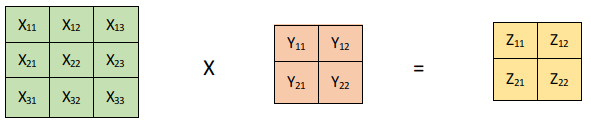
\includegraphics[width=0.8\textwidth]{./hinhanh/chap3/conv_operation.png}}
		\caption{Example of convolution operation.}
	\end{figure}
	
	Calculation step as below:
	\[Z_{11} = X_{11}Y_{11} + X_{12}Y_{12} + X_{21}Y_{21} + X_{22}Y_{22}\]
	\[Z_{12} = X_{11}Y_{12} + X_{12}Y_{13} + X_{21}Y_{22} + X_{22}Y_{23}\]
	\[Z_{21} = X_{11}Y_{21} + X_{12}Y_{22} + X_{21}Y_{31} + X_{22}Y_{32}\]
	\[Z_{22} = X_{11}Y_{22} + X_{12}Y_{23} + X_{21}Y_{32} + X_{22}Y_{33}\]
	
	This process seems simple, but it is very effective in image processing. In a CNN, the input is a tensor with shape (number of images) x (image height) x (image width) x (input channels). After passing through a convolution layer, the image becomes abstracted to a feature map (the result after applying convolution operation), with shape (number of images) x (feature map height) x (feature map width) x (feature map channels).
	
	To train or modify a CNN, there are some attributes we should keep track on:
	\begin{itemize}
		\item The size and the number of filters/kernels (hyper-parameters).
		\item The number of input and output channels (hyper-parameters).
		\item The quantity of filters is equal to the quantity of feature maps.
		\item Padding and Stride attributes in convolution operations.
	\end{itemize}

	Padding and Stride are the crucial technique in convolution. Let’s take a look at the previous example in Figure 1. We calculated the feature map by sliding the filter on the input data by one pixel for each convolution operation, we refer to the number of rows and columns traversed per slide as the stride. The smaller step we define in filters, the more information we can extract from it, but it is a trade-off which affect the training time. One tricky issue when applying convolution layers is that we tend to lose pixel information on the perimeter of input data.
	
	\begin{figure}[H]
		\centering
		{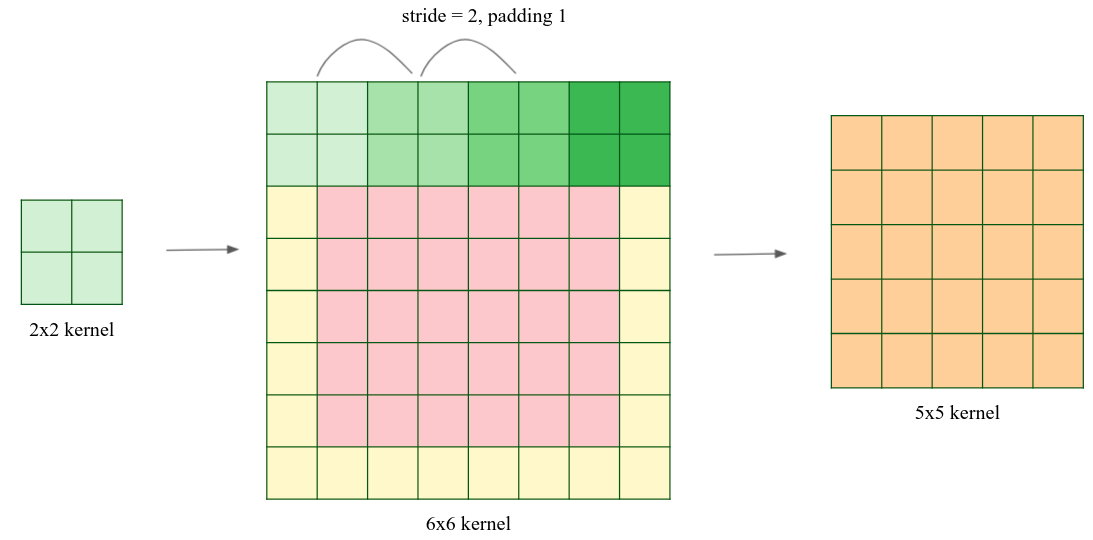
\includegraphics[width=0.8\textwidth]{./hinhanh/chap3/padding.png}}
		\caption{Missing pixels information when doing convolution.}
	\end{figure}

	This problem happens when we slide the filter on input data, our filters only do convolution operation on pixels at the edge of matrix fewer than pixels which are close to the center of the matrix. Even though, it is just a few pixels, we use lots of convolution layers, it will add up and cause missing information. That is why the term “Padding” comes up, a direct solution for this is to add a “barrier” of zero pixels surrounding the input matrix which increases the effective size of the input matrix.
	
	\begin{figure}[H]
		\centering
		{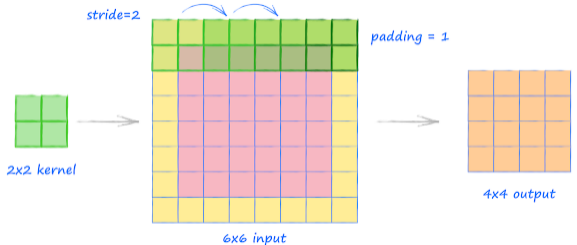
\includegraphics[width=0.8\textwidth]{./hinhanh/chap3/zero_padding.png}}
		\caption{Applying zero padding = 1 to the input matrix.}
	\end{figure}
	
\subsubsection{Pooling layer}
\noindent

	As described in previous section, the convolutional layer output is a feature maps, as it can be regarded as the learned representations (features) in the spatial dimensions (e.g., width and height) to the subsequent layer. Usually, as we process an image, we want to reduce the spatial resolution of our feature maps, select information so that it can be more robust or sensitive when we go deeper in the network.  By gradually aggregating information, yielding coarser and coarser maps, our model can accomplish a global representation for the feeding dataset.
	
	Like convolution, pooling operator consists of a fixed-shape window that slide all over on the output feature map according to its stride setting. However, unlike sliding window of convolutional layer, sliding window of pooling layer does not have any parameters (no kernel). Instead of calculating the feature map, pooling layer simply calculate either the maximum or average value of the pixels inside its sliding window. These operations are called maximum pooling and average pooling, respectively. Another characteristic of  pooling layer is that it also can alter padding and stride settings to prevent model from missing information. 	
	
	\begin{figure}[H]
		\centering
		{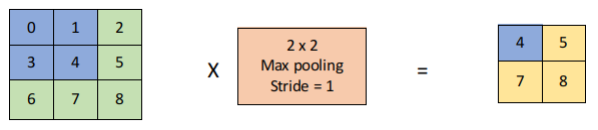
\includegraphics[width=0.8\textwidth]{./hinhanh/chap3/max_pooling.png}}
		\caption{Max pooling with window shape 2x2 and stride = 1.}
	\end{figure}
	
\subsubsection{Fully connected layer}
\noindent

	Fully-connected (FC) layers connect every neuron in one layer to every neuron in another layer. It is the similar to a traditional multi-layer perceptron neural network (MLP). After we extract feature maps from convolutional layers, we flatten these maps to one dimension vector and then feed it to the FC layer for the model to learn how to classify the data. However, FC layers can be seen as a brute force approach whereas there are approaches like the convolutional layer which reduces the input to concerned features only. That is the reason why CNN models are often built with few FC layers (one or two layers).	
	
\subsubsection{Loss function}
\noindent

	In the training process, a CNN model learns to map a set of inputs to a set of outputs. By using gradient-based training method, the mapping process cannot be calculated perfectly in one step due to convergence process. Therefore, the model has to feed the inputs from the dataset over and over again to improve the mapping result. As a result, the problem of learning is explore as optimization problem. 
	
	Base on this idea, loss function (or cost function) is defined as the difference of the dataset output and the predicted output of the model. It is like a form of getting the model to pay a penalty after a wrong prediction, and loss function output is proportional to the severity of the error. In supervised learning problem, the goal is to minimize this loss as low as possible (In the ideal condition, loss function returns 0).
	
	A general loss function is expressed as below:
	\[
	L_\varepsilon\bigl(y,f(x,w)\bigr)=
	\begin{cases}
	0 & \bigl|y-f(x,w)\bigr|\leq\varepsilon,\\
	\bigl|y-f(x,w)\bigr|-\varepsilon & \text{otherwise},
	\end{cases}
	\]
	
	As loss function calculate the difference between the right and the wrong mapping value, naturally, it can be defined as a subtraction of the two values. However, subtracting 2 values may result in negative number which cannot be considered, therefore, an absolute expression is added to constrained its output.
	
	\[L(\hat{y}\,y) = | \hat{y}\ - y | \]
	
	Because the model is trained based on gradient based method, the minimization process of above function is hardly to achieve due to the un-continuous derivative (for example, derivative of $f(x) = |x|$ is interrupted at 0). To address this issue, the whole expression is squared and then divide by two.
	
	A simple loss function:
	\[L(\hat{y}\,y) = \frac{1}{2}\ (\hat{y}\ - y)^2 \]
	
	Let's take a binary classification problem to be an simple example which $\hat{y}\ < 0$ means the model prefers -1 prediction and $\hat{y}\ > 0$ means the model prefers 1 prediction. Hence, an appropriate loss function that satisfies the following criteria:
	
	1. Whenever the model make a wrong predict, it must be punished badly. Therefore, the first criteria is that loss function has to return a bigger value if $\hat{y}$ is opposite to $y$ than the contrast.
	
	2. If there are two answers $\hat{y}$ and $y$ both have the same sign (or different sign), which one should be punished more? As mentioned before, the absolute value $| \hat{y}\ |$ represents the "prefer-ness" of the model for an option. The larger this value, the more the model prefers an answer. In the case of the same sign, the preferred option is the correct one, so the more the model likes its prediction, the less penalties must be paid. With the same argument, if the sign $ \hat{y}\ $ is different from $y$, because the preferred option is the wrong one, the more the model likes, the more severe penalties will be imposed on the model so that the model will not repeat it. 

	Yet, with different problems, there are different loss functions with multiple criteria. Therefore, before applying any models, algorithms, researchers need to identify the problem so that they can choose a suitable loss function to train the model.

\subsubsection{Optimization function}
\noindent

	In the previous section, we discussed about the loss function and its criteria. Once we define a loss function to make penalty on the wrong prediction of the model, we need to minimize the loss value in attempt to make the model prediction better after each training step. Therefore, an algorithm called optimization algorithm was brought into the training process in order to serve the optimization problem in the training phrase.
	
	Although optimization provides a way to minimize the loss function for deep learning, in essence, the goals of optimization and deep learning are fundamentally different. The former is primarily concerned with minimizing an objective whereas the latter is concerned with finding a suitable model, given a finite amount of data.
	
	Despite the fact that optimization algorithm provides a method for deep learning model to minimize the loss function value, in general, the purpose of them is essentially different from one another. In deep learning field, we mostly concern find a model that can generalize a finite amount of given data. However, the goal of optimization is to minimize the objective function.
	
	To be more specific, training error and generalization error are ordinarily different:

	1. As the objective function of optimization algorithm is often a loss function, so its goal is to decrease the error in the training process.

	2. In deep learning or statistical field, the goal is to reduce generalization error.

	To accomplish the latter we need to pay attention to over-fitting in addition to using the optimization algorithm to reduce the training error \cite{dive2dl}.
	
	There lots of problems when we try to optimize loss function of a deep learning model. Therefore, in this section, we will focus on several controversial issues such as local minima, saddle point, gradient exploding and gradient vanishing.
	
	As mentioned in loss function section, gradient-base method is mostly apply to train a deep learning model using backpropagation algorithm. Hence, in the process of training a model, the derivative calculation is done continuously and throughout to find the global minimum point of the function representing the data set - $ f (x) $. For ease of visualization, we will look at figure 3.7.
	
	\begin{figure}[H]
		\centering
		{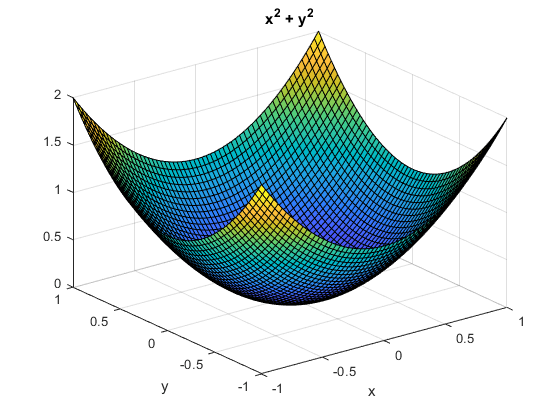
\includegraphics[width=0.7\textwidth]{./hinhanh/chap3/bowl_shape.png}}
		\caption[bowl]{Bowl shape function - $ \ {x^2} + {y^2} \ $.}
	\end{figure}
	
	Assuming this cup-shaped plane is the equation f (x), its minimum point will be in the center of the cup. If we jump into this plane, of course we will slip straight to its minimum point. So when a function converges at its minimum, it optimizes as much as possible in the ability to classify the data. This is the fundamental goal of training: to continue modifying weights until the global minimum has been reached.
	
	However, not all functions are cup-shaped. Let's take a look at figure 3.8 below for easier visualization.
	
	\begin{figure}[H]
		\centering
		{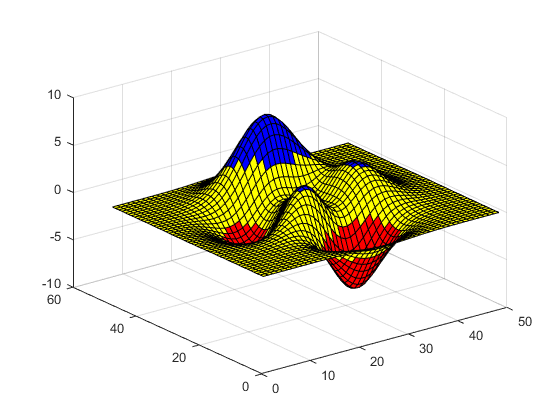
\includegraphics[width=0.8\textwidth]{./hinhanh/chap3/global.png}}
		\caption{Local minima and global minima.}
	\end{figure}
	
	A function of the deep learning model usually takes the same form for many local minima points. Then, the function is susceptible to convergence at local minima points because it can only optimize the function of the model locally. This causes the gradients to be zero early and adversely affects the model's training and its results.
	
	Besides local minima, saddle points are also a cause which make gradient vanish early. Although saddle point can cause gradient vanishing, it is not neither local minima nor global minima. 
	
	\begin{figure}[H]
		\centering
		{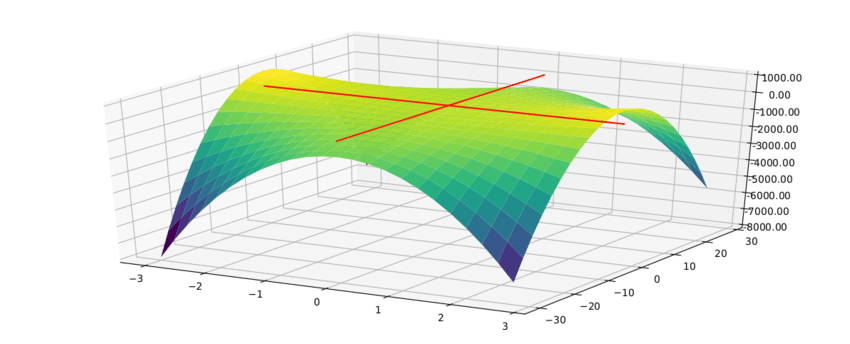
\includegraphics[width=0.9\textwidth]{./hinhanh/chap3/saddle.png}}
		\caption{Saddle point.}
	\end{figure}
	
	
\section{Gradient descent}
	\noindent
	
	In deep learning in particular and optimization math in general, we often have to find the smallest value of a function. However, finding the global minima of loss functions in deep learning is very complicated or even impossible. Instead, people often try to find the local minima points, and to a certain extent, consider it the solution to be found in the problem.
	
	The local minima points are the solutions of the derivative equation equal to 0. If it is possible to find the whole (finite) minimum points, we can replace each of those local minimum points into the objective function and then find the point making it the smallest value. 
	
	Yet, in most cases it is not possible to solve zero derivative equations. The cause can come from the complexity of the derivative form, from the fact that the data points have a large number of dimensions (Look at figure bla bla for more detail).
	
	\begin{figure}[H]
		\centering
		{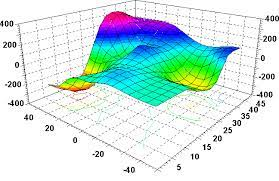
\includegraphics[width=0.5\textwidth]{./hinhanh/chap3/flutuate_plate.jpg}}
		\caption{It is hard for GD to be converging at global minima.}
	\end{figure}
	
%	\begin{figure}[H]
%		\centering
%		\subcaptionbox{Gradient descent in a perfect condition.}{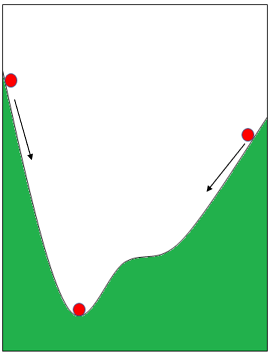
\includegraphics[width=0.3\textwidth]{./hinhanh/chap3/GD.png}}%
%		\hfill % <-- Seperation
%		\subcaptionbox{Gradient descent is stuck at local minima.}{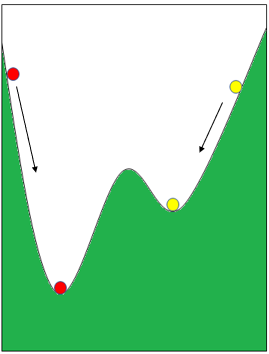
\includegraphics[width=0.3\textwidth]{./hinhanh/chap3/GD-2.png}}%
%		\hfill % <-- Seperation
%		\subcaptionbox{Gradient descent with momentum overcome local minima.}{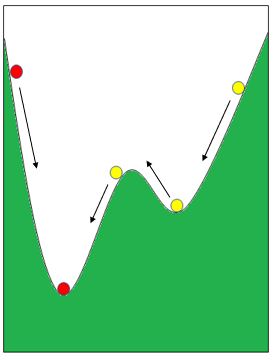
\includegraphics[width=0.3\textwidth]{./hinhanh/chap3/GD_momentum.png}}%
%		\hfill % <-- Seperation
%		\caption{Gradient descent versus Gradient descent with momentum.}
%	\end{figure}
	
	The most typical approach is to start from a point that we consider to be close to the global minima, then use an iteration to move closer to the desired point. Gradient Descent (GD) and its variations are among the most popular methods.
	
	In this part, we will take gradient descent in one dimension as a simple example to explain it functional mechanism. Let assume we have a function as follow.
	
	\[f(x) = \frac{1}{2} \cdot (x - 1)^2 -2\]
	
	Supposed $x_t$ is the point that we find after the $t$-th iteration. The goal is to define a function that can bring $x_t$ as close as possible to the global minima after a specific number of iteration.
	
	\begin{figure}[H]
		\centering
		{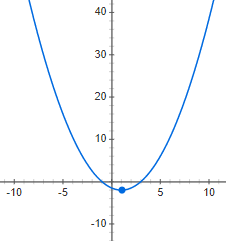
\includegraphics[width=0.3\textwidth]{./hinhanh/chap3/simple_f(x).png}}
		\caption{$ f(x) = \frac{1}{2} \cdot (x - 1)^2 -2 $.}
	\end{figure}
	
	Look at the plot of the objective function. It is noticeable that if the derivative of the objective function at $x_t$ is greater than zero, $x_t$ will stay on the right compared to the global minima and contrast. Therefore, to bring $x$ closer to the goal, it is needed to be moved toward the left side of the minima which means the negative side. In other word, $x_t$ has to move oppositely to the derivative.  
	
	\[x_{t+1} = x_t + \Delta \] $\Delta$ is a quantity opposite to the derivative $f'(x)$
	
	\noindent	
	The farther away $x_t$ is from x to the right, the larger $f(x_t)$ and vice versa. Therefore, delta is proportional to $-f'(x_t)$.
	\noindent	
	As a result, the equation is represented as following:
	
	\[x_{t+1} = x_t - \eta \cdot f'(x_t)\]
	
	Where $\eta$ is a positive number called learning rate. The minus shows that it has to move oppositely to the derivative. It is the reason why this method is called Gradient Descent (means moving backward). In conclusion, the constructing of the function above, even though it is not always reasonable for all problems, it is a foundation for lots of optimization approach in general and deep learning in particular.
	
	\section{Multivariate gradient descent}
	\noindent
	
	Let say we need to find global minima cho the function $f(\theta)$ that $\theta$ is a vector usually used to denote the set of parameters (or weights) of the objective function. The derivative of the function at any $\theta$ is denoted as $\nabla_{\theta}f(\theta)$. It is similar to one variable function, GD for multivariate is also started at a predicted point $\theta_0$. After that, it is updated as following:
	
	\[\theta_{t+1} = \theta_t - \eta\nabla_{\theta}f(\theta_t) \]
	
	\noindent	
	Or it is simply represented as:
	
	\[\theta = \theta - \eta\nabla_{\theta}f(\theta) \]
	
	\noindent
	Note: Always move oppositely to the derivative.
	
\section{Gradient descent variants}
	\noindent
	
	In general, there are in total three variants of GD algorithm. Each of them has has a unique approach on using the amount of data to calculate the derivative of the objective function. Therefore, the amount of data used will affect directly on the convergence speed of the derivative and may cause a trade-off between the accuracy and the time on each update of the weights.
	
	
	\subsection{Batch gradient descent}
	\noindent

	The GD algorithm is mentioned from the beginning of GD section is the vanilla one - batch gradient descent. In this circumstance, the word "batch" means "all" which means all of the data $x_i$ are used whenever an update is perform on the weights $\theta = w$. Therefore, this technique shows that computation in training process is effectively due to no update required after each training sample.
	
	This vanilla approach works ineffectively if there is a huge dataset. Because it has to calculate gradient and update weights for all data in the dataset after each epoch which slowdown the training process.
	
	\subsection{Stochastic gradient descent}
	\noindent

	In deep learning, the objective function is usually the average of the loss functions for each example in the training dataset. By using SGD, at a time, only one data point $x_i$ is used to calculate gradient and then it updates the weights -  $\theta$. This work is executed with each data point in the whole dataset and repeated after each epoch. 
	
	\[\theta = \theta - \eta \nabla_{\theta} J(\theta; x_i; y_i)\]
	
	\noindent
	$ J(\theta; x_i; y_i)$ is a loss function with the input is a pair data (input, label).
	
	With normal GD, each epoch corresponds to 1 update $\theta$, but with SGD, each epoch corresponds to $N$ update $\theta$ ($N$ is the number of data points in the dataset). Look at one hand, updating is executed on each data point may lead to a slow training epoch. Look at the other hand, SDG only requires a few epoch to complete its training process. Therefore, SGD is suitable for a huge dataset rather than the vanilla one.
	
	Yet, due to the frequent updates, the steps taken towards the minima are very noisy. This can often lean the gradient descent into other directions or may not settle on global minima. Moreover, SGD is not only expensive in computation because of using all resources to train, but it also loses the advantage of vectorized operations as it deals with only one data sample at a time
	
	
	\subsection{Mini-batch gradient descent}
	\noindent
	
	Similar to SGD, mini-batch GD uses $n$ data points (greater than 1 and smaller than the whole dataset). Mini-batch GD starts each training epoch by shuffle all data points and divides them into small batches. Each of them has $n$ data points (except for the last batch may have fewer if $N$ is not divisible to $n$) At each update, mini-batch GD takes one batch to calculate gradient and updates it as following.
	
	\[ \theta = \theta - \eta \nabla_{\theta} J(\theta; x_i; y_i) \]
	
	\noindent
	By taking the advantages of both original GD and SDG, mini-batch GD shows its computational efficiency (compared to the vanilla GD), stable convergence towards global minima, and faster learning as it calculate gradient on multiple data samples and update the weights more regularly (compared to SGD).
	
	As a result, mini-batch GD has been applied widely in machine learning field, especially in deep learning.

\section{Adam optimization}
	
	
	